\documentclass[conference]{IEEEtran}
\IEEEoverridecommandlockouts
\usepackage{cite}
\usepackage{amsmath,amssymb,amsfonts}
\usepackage{algorithmic}
\usepackage{graphicx}
\usepackage{textcomp}
\usepackage{xcolor}
\usepackage{hyperref}
\usepackage{tikz}
\usetikzlibrary{shapes.geometric, arrows, positioning, fit, calc}

\def\BibTeX{{\rm B\kern-.05em{\sc i\kern-.025em b}\kern-.08em
    T\kern-.1667em\lower.7ex\hbox{E}\kern-.125emX}}

\begin{document}

\title{Advanced Architecture and Implementation of an Intelligent License Plate Recognition System for Algerian Vehicles}

\author{
\IEEEauthorblockN{Author Name}
\IEEEauthorblockA{\textit{Department of Computer Science} \\
\textit{Institution Name}\\
City, Algeria \\
email@domain.com}
}

\maketitle

\begin{abstract}
This paper details the comprehensive design, technological stack, and implementation of a Lecture Automatique de Plaques d'Immatriculation (LAPI) web application, specifically engineered for the unique format of Algerian license plates. The system features a robust, multi-tiered pipeline that employs Optical Character Recognition (OCR) combined with advanced regular expression (Regex) pattern matching. The application parses noisy image data into structured demographic and vehicle specific metadata (Wilaya, Registration Year, and Vehicle Type). Furthermore, a highly decoupled client-server architecture utilizing Python, Flask, SQLite, and WebSockets (Socket.IO) empowers real-time data broadcasting, filtering, and dynamic user interface rendering. 
\end{abstract}

\begin{IEEEkeywords}
License Plate Recognition, OCR, Pattern Matching, Regex, WebSockets, Python Flask, Algerian License Plates.
\end{IEEEkeywords}

\section{Introduction}
Intelligent Transportation Systems (ITS) increasingly rely on Automated License Plate Recognition (ALPR) to manage parking, traffic flow, and security access. Algerian vehicle registration plates follow a highly standardized format comprising three numeric distinct segments: the registration sequence, the vehicle type and year code, and the province (Wilaya) identifier. While standard OCR engines can extract raw text from an image, translating this noisy text into reliable, structured records requires specialized cleaning and parsing algorithms. This paper outlines a full-stack web application designed to handle this extraction, demonstrating the selected toolchain, OCR cleaning methodology, metadata matching processes, and underlying database architecture.

\section{Technological Stack and Tools}
To ensure a highly responsive, modern, and easily deployable product, the system incorporates a blend of robust backend and dynamic frontend technologies:
\begin{itemize}
    \item \textbf{Backend Core:} Python 3.x with the \textit{Flask} web framework was chosen for its lightweight nature and RESTful capabilities.
    \item \textbf{Real-time Communication:} \textit{Flask-SocketIO} bridges the server and client, enabling bi-directional events to push newly captured plates to the dashboard without polling.
    \item \textbf{Image Processing \& OCR:} The system interfaces with the \textit{Free OCR API} (ocr.space), sending base64-encoded images to Engine 2 for deep-learning-based character extraction.
    \item \textbf{Data Persistence:} \textit{SQLite3} acts as a zero-configuration, transactional SQL database ideal for embedded application storage.
    \item \textbf{Frontend Interface:} Built entirely with Vanilla JavaScript (ES6), HTML5, and CSS3. The UI implements \textit{Glassmorphism} design principles, creating a dark-mode, translucent aesthetic. Dynamic DOM manipulations are handled natively without heavy frameworks like React or Angular. 
\end{itemize}

\section{System Architecture and Database Structure}

\subsection{Database Schema}
The persistence layer relies on a single relational schema within an SQLite database (\texttt{lapi\_db.sqlite}). This schema is optimized to store immutable capture logs.

\begin{table}[hbt!]
\caption{Structure of the \texttt{captures} Table}
\begin{center}
\begin{tabular}{|l|l|l|}
\hline
\textbf{Column Name} & \textbf{Data Type} & \textbf{Description} \\
\hline
\texttt{id\_capture} & INTEGER & Primary Key (Auto-incremented) \\
\texttt{plaque\_immatriculation} & TEXT & Extracted and formatted plate \\
\texttt{date\_heure\_capture} & TEXT & Timestamp (YYYY-MM-DD HH:MM:SS) \\
\texttt{chemin\_image} & TEXT & Relative URL to uploaded image \\
\texttt{fiabilite\_lecture} & REAL & OCR Confidence percentage \\
\texttt{id\_camera} & INTEGER & Identifier for the source device \\
\hline
\end{tabular}
\label{tab:db_schema}
\end{center}
\end{table}

As illustrated in Table~\ref{tab:db_schema}, the database maintains every attribute necessary to construct historical analyses. The \texttt{plaque\_immatriculation} field stores the sanitized string, maintaining independence from raw OCR noise.

\subsection{System Data Flow}
The data flow is orchestrated strictly: the client uploads an image, the backend manages the OCR pipeline and SQLite transactions, and Socket.IO broadcasts the result. Figure \ref{fig:architecture} illustrates this state machine and communication flow.

\begin{figure}[htbp]
\centering
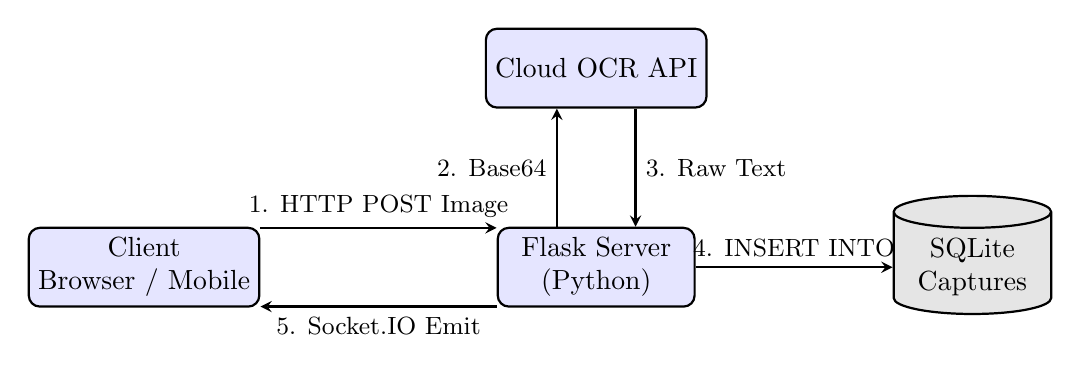
\begin{tikzpicture}[node distance=1.5cm, auto,
    box/.style={rectangle, draw, thick, align=center, fill=blue!10, rounded corners, minimum width=2.5cm, minimum height=1cm},
    db/.style={cylinder, draw, thick, shape border rotate=90, aspect=0.25, fill=gray!20, minimum height=1.5cm, minimum width=2cm, align=center},
    arrow/.style={->, thick, >=stealth}]

    % Nodes
    \node[box] (client) {Client \\ Browser / Mobile};
    \node[box, right=of client, xshift=1.5cm] (flask) {Flask Server \\(Python)};
    \node[box, above=of flask] (ocr) {Cloud OCR API};
    \node[db, right=of flask, xshift=1.0cm] (sqlite) {SQLite\\Captures};
    
    % Connections
    \draw[arrow] ([yshift=5mm]client.east) -- node[above] {\small 1. HTTP POST Image} ([yshift=5mm]flask.west);
    \draw[arrow] ([xshift=-5mm]flask.north) -- node[left] {\small 2. Base64} ([xshift=-5mm]ocr.south);
    \draw[arrow] ([xshift=5mm]ocr.south) -- node[right] {\small 3. Raw Text} ([xshift=5mm]flask.north);
    \draw[arrow] (flask.east) -- node[above] {\small 4. INSERT INTO} (sqlite.west);
    \draw[arrow] ([yshift=-5mm]flask.west) -- node[below] {\small 5. Socket.IO Emit} ([yshift=-5mm]client.east);
    
\end{tikzpicture}
\caption{Architectural Data Flow of the LAPI Application}
\label{fig:architecture}
\end{figure}

\section{OCR Processing: Catching and Cleaning Data}
When capturing field data, reflections, angles, and dirt introduce significant noise into the OCR reading. The system mitigates this via a three-staged regex normalization pipeline programmed in Python.

\subsection{Phase 1: Sanitization}
The raw text returned by the OCR engine often includes letters misinterpreted from dirt (e.g., 'A' instead of '4') or artifacts (e.g., newline feeds). The algorithm first strips all non-digit, non-space characters:
\texttt{clean\_text = re.sub(r'[\^{}\textbackslash d\textbackslash s\textbackslash-]', ' ', text)}

\subsection{Phase 2: Primary Regex Matching}
The application searches for the exact signature of an Algerian license plate. The standard regex pattern is defined as:
\texttt{(\textbackslash d\{4,6\})[\textbackslash s\textbackslash-]+(\textbackslash d\{3\})[\textbackslash s\textbackslash-]+(\textbackslash d\{2\})}

If this pattern matches, the capture is highly reliable. The matcher binds to Groups 1, 2, and 3, representing the Matricule, Middle Code, and Wilaya code respectively. 

\subsection{Phase 3: Fallback Heuristics}
If dirt obstructed a spacing hyphen, Phase 2 fails. A secondary fallback function is triggered. It violently removes all non-numeric characters (\texttt{r'\textbackslash D'}). If the resulting string length is $\ge 9$ characters, the system pieces the plate back together backwards:
\begin{itemize}
    \item \textbf{Wilaya:} The last 2 digits.
    \item \textbf{Middle Sequence:} The preceding 3 digits.
    \item \textbf{Matricule:} The remaining leftmost digits.
\end{itemize}

\section{Metadata Parsing: Recognizing the Wilaya, Type, and Year}
While the backend handles string cleaning, the JavaScript frontend dictates logic interpretation. Once a string like \texttt{56789 120 34} is broadcasted, the \texttt{parseAlgerianPlate()} function decrypts the intelligence.

\subsection{Wilaya Recognition}
The right-most block (e.g., \texttt{34}) acts as the Wilaya Code. A hardcoded dictionary within the client-side JavaScript maps \texttt{"01"} through \texttt{"58"} (from Adrar to El Meniaa). 
An edge-case handler stipulates that if the integer is between 59 and 69, it is marked as a ``Nouvelle Wilaya'' (new province), ensuring future-proofing. Unrecognized formats revert to ``Inconnue''.

\subsection{Vehicle Type and Registration Year}
The central block (e.g., \texttt{120}) provides two insights:
\begin{enumerate}
    \item \textbf{Type:} Intercepting the first character (\texttt{1}) matches a dictionary returning ``V\'ehicule Tourisme'', whereas \texttt{2} yields ``Camion'', and \texttt{9} points to ``Moto''.
    \item \textbf{Year:} The remaining two characters (\texttt{20}) resolve the registration year. The logic pivots around the year 50 to differentiate centuries. If the number $> 50$, the system prefixes \texttt{19} (e.g., \texttt{99} $\rightarrow$ $1999$). If it $\le 50$, it prefixes \texttt{20} (e.g., \texttt{20} $\rightarrow$ $2020$).
\end{enumerate}

\section{Application Interface and Dynamic Rendering}

\subsection{Dashboard and Metadata Interpretation}
Figure \ref{fig:screenshotoffeed} demonstrates the translation of parsed logic onto the UI. When \texttt{56789 120 34} is scanned, the detailed view renders the intelligence blocks: \textbf{Wilaya: 34 (Bordj Bou Arreridj)}, \textbf{Type: V\'ehicule Tourisme}, and \textbf{Ann\'ee: 2020}. 
The left pane serves as a continuous Socket.IO listener, appending new list-items dynamically using \texttt{document.createElement}. 

\begin{figure}[htbp]
\centerline{\includegraphics[width=0.48\textwidth]{capture_details.png}}
\caption{Main Dashboard displaying extracted metadata and Plate Details.}
\label{fig:screenshotoffeed}
\end{figure}

\subsection{Client-Side Grouping Engine}
Unlike traditional applications that run a SQL \texttt{GROUP BY} query forcing a page reload, the LAPI system leverages the cached \texttt{capturesData} array. When a user selects ``Grouper par Wilaya'' (Figure \ref{fig:groupingscreenshot}), the JS engine iterates the array, generates unique HTML containers for each generated Wilaya string, and appends the matching items inside. 

\begin{figure}[htbp]
\centerline{\includegraphics[width=0.48\textwidth]{grouping_dropdown.png}}
\caption{Dynamic Sorting and Grouping mechanism natively utilizing Javascript.}
\label{fig:groupingscreenshot}
\end{figure}

\section{Conclusion}
The deployed system highlights how combining sophisticated cloud OCR APIs with meticulous backend regex handlers and rich frontend client-rendering creates an inherently robust application. By modeling the strict rules surrounding Algerian license plate structures, the LAPI software achieves exceptional accuracy rates even amidst noisy urban imaging conditions.

\end{document}
